% !TEX program = xelatex
% !TEX TS-program = xelatex
% !TEX encoding = UTF-8 Unicode

\documentclass[a4paper, 12pt]{article}
\usepackage{amsmath}
\usepackage{fontspec}  % 解决中文问题
	\defaultfontfeatures{Mapping=tex-text}
	\setromanfont{Songti SC}  % Mac下使用此句
	% \setromanfont{"[msyh.ttc]"}  % Windows下使用此句
	\XeTeXlinebreaklocale “zh”
	\XeTeXlinebreakskip = 0pt plus 1pt minus 0.1pt
\usepackage[top=20mm, bottom=25mm, left=20mm, right=25mm]{geometry}  % 设置页边距
	% \special{papersize=12cm,9cm}  % For Kindle
	% \setlength\paperheight{35cm}  % For iPhone 7
	% \setlength\paperwidth{20cm}
\usepackage{tikz}  % 画图用s
	\def\pgfsysdriver{pgfsys-dvipdfmx.def}
\usepackage{xltxtra}
\usepackage{xunicode}

\renewcommand{\thefootnote}{注[\arabic{footnote}]}  % 重新定义\footnote命令的格式


\usepackage[colorlinks,linkcolor=blue]{hyperref}  % 设置超链接

\graphicspath{{../}}



\begin{document}
	\title{机器学习笔记}
\author{MingShun Wu}
\date{\today}
\maketitle
	\renewcommand{\contentsname}{目录}
\tableofcontents
\setcounter{tocdepth}{3}
	\section{前言}
\begin{enumerate}
	\item 本人也是初学者,一下内容均为自己的学习笔记,可能有很多错误,若有错误可联系我。本人微信二维码如下。
	\begin{figure}[htbp]
		\centering
		
\includegraphics[scale=0.3]{images/微信号二维码}
		\caption{微信号二维码}
	\end{figure}
\end{enumerate}





























	\section{线性回归}
\subsection{假设函数(Hypothesis Function)}
\begin{equation}\begin{aligned}
	h_\theta(x) = \theta_0 + \theta_1x_1 + \theta_2x_2 + \theta_3x_3 + ... + \theta_nx_n
\end{aligned}\end{equation}
另$x_0=1$,则
\begin{equation}\begin{aligned}
	h_\theta(x) &= \theta_0x_0 + \theta_1x_1 + \theta_2x_2 + \theta_3x_3 + ... + \theta_nx_n \\
	&= \sum_{j=0}^n{\theta_jx_j}
\end{aligned}\end{equation}

\subsection{最小二乘法}
梯度下降中的Cost Function均使用的时最小二乘法

\subsection{梯度下降}
\subsubsection{批梯度下降(BGD)}
\begin{enumerate}
	\item Cost Function
	\begin{equation}\begin{aligned}
		J(\theta) = \frac{1}{2} \sum_{i=1}^m \left[h_{\theta} {(x^{(i)})} - y^{(i)}\right]^2
	\end{aligned}\end{equation}
	其中,$J(\theta)$就是在训练过程中的Cost Function。我们的目的就是将该Cost Function最小化。
	在以上式子中:\\
		$x^{(i)}$为训练集的输入;\\
		$y^{(i)}$为训练集的输出;\\
		$\theta$为所要训练的参数;\\
		$h_{\theta}$为假设函数;\\
		$h_{\theta} {(x^{(i)})}$为训练集输入经过假设函数后得到的结果\\
		以上式子中,其实是使用最小二乘法

	\item 迭代方式
	\begin{equation}\begin{aligned}
	      \theta_j &:= \theta_j - \alpha \frac{\partial} {\partial \theta_j} J(\theta)
	\end{aligned}\end{equation}
	其中:
	\begin{equation}\begin{aligned}
	      \frac{\partial} {\partial \theta_j} J(\theta) &= \frac{\partial}{\partial \theta_j} \frac{1}{2} \sum_{i=1}^m\left[ h_\theta(x^{(i)}) - y^{(i)} \right]^2 \\
	      &= 2 * \frac{1}{2} \sum_{i=1}^m\left[ h_\theta(x^{(i)}) - y^{(i)} \right] \frac{\partial}{\partial\theta_j}\left[ h_\theta(x^{(i)}) - y^{(i)} \right] \\
	      &= \sum_{i=1}^m\left[ h_\theta(x^{(i)}) - y^{(i)} \right]\frac{\partial}{\partial\theta_j}\left[ \theta_0x_0^{(i)} +  \theta_1x_1^{(i)} + \theta_2x_2^{(i)} + ... + \theta_nx_n^{(i)} - y^{(i)} \right] \\
	      &= \sum_{i=1}^m\left[ h_\theta(x^{(i)}) - y^{(i)} \right]x_j^{(i)}
	\end{aligned}\end{equation}
	所以,更新后的梯度下降公式为
	\begin{equation}\begin{aligned}
		\theta_j &:= \theta_j - \alpha \sum_{i=1}^m \left[ h_\theta(x^{(i)}) - y^{(i)} \right]x_j^{(i)}
	\end{aligned}\end{equation}
	其中,$\alpha$称为学习速率(learning rate),用于控制$\theta$前进的步伐,避免$\theta$走得太快(或太慢)。\\

	梯度下降法每次计算都是找到当前所在位置中,下降最快的方向(至于为什么是当前所在位置中下降最快的方向就是梯度的定义了)。 \\
	如果计算进入了某个局部极小值,则很可能一直在这个局部极小值内出不来了(除非你的步长比较大,帮助它跑出这个局部极小值),这就是梯度下降法的局限所在,它很容易陷入局部极小值中。 \\
	使用梯度下降法每次修正的时参数$\theta$,而不是输入的$X$或$y$ \\

	Todo PS: 以下内容正确性待思考。因为其是当前位置下,下降最快的方向,若出现每个维度求导后结果都是0,则此时不论再怎么迭代,这个点都不会再变化了(或者其他导致每个维度的偏导数都为0的情况也类似,当然,这种情况较少见)
\end{enumerate}


\subsubsection{随机梯度下降(SGD)}
由批梯度下降的式子可以发现,在每一次梯度下降的迭代过程中,我们遍历了所有训练集。这将会耗费大量的性能,于是产生了随机梯度下降(SGD)方法,每次迭代只使用一个数据。 \\
\begin{enumerate}
	\item Cost Function
	\begin{equation}\begin{aligned}
		J(\theta) = \frac{1}{2} \left[h_{\theta} {(x^{(i)})} - y^{(i)}\right]^2
	\end{aligned}\end{equation}

	\item 迭代方式
	\begin{equation}\begin{aligned}
	      \frac{\partial} {\partial \theta_j} J(\theta) &= \left[ h_\theta(x^{(i)}) - y^{(i)} \right]x_j^{(i)}
	\end{aligned}\end{equation}
	更新后的梯度下降公式为
	\begin{equation}\begin{aligned}
		\theta_j &:= \theta_j - \alpha\left[ h_\theta(x^{(i)}) - y^{(i)} \right]x_j^{(i)}
	\end{aligned}\end{equation}
	如上所示,与批梯度下降不同,随机梯度下降每次迭代只用了一个数据(第$i$个数据),若$i$从1取到m,则完成了一次训练集的遍历。\\
	使用随机梯度下降虽然解决了批梯度下降耗费过多性能的问题,但是却带来了另一个问题:收敛太慢!由此,我们折中使用迷你批梯度下降(mini-batch GD)。\\
	随机梯度下降(包括其他梯度下降方法)均允许多次遍历所有数据集。
\end{enumerate}

\subsubsection{迷你批梯度下降(mini-batch GD)}
为了解决梯度下降每次都使用所有训练集导致的性能问题,以及随机梯度下降每次只使用一个数据导致的收敛太慢,我们可以只用mini-batch GD。每次只用一部分训练集进行训练。
\begin{enumerate}
	\item Cost Function \\
	略

	\item 迭代方式 \\
	略
\end{enumerate}











		\subsection{线性代数知识}
\begin{enumerate}
	\item
	\begin{equation}
		\nabla_{\theta}J(\theta) = \left[\begin{matrix}
		\frac{\partial J}{\partial\theta_0} \\
		\frac{\partial J}{\partial\theta_1} \\
		\vdots \\
		\frac{\partial J}{\partial\theta_n} \\
		\end{matrix}\right], \quad \in {\rm I\!R}^{n+1}
	\end{equation}

	\item
	\begin{equation}
		\nabla_Af(A) = \left[ \begin{matrix}
			\frac{\partial f}{\partial A_{11}} & \frac{\partial f}{\partial A_{12}} & \dots & \frac{\partial f}{\partial A_{1n}} \\
			\frac{\partial f}{\partial A_{21}} & \frac{\partial f}{\partial A_{22}} & \dots & \frac{\partial f}{\partial A_{2n}} \\
			\vdots & \vdots & \ddots & \vdots \\
			\frac{\partial f}{\partial A_{n1}} & \frac{\partial f}{\partial A_{n2}}& \dots & \frac{\partial f}{\partial A_{nn}} \\
		\end{matrix}\right]
	\end{equation}

	\item 矩阵的迹的计算方式 \\
	如果矩阵$A$是方阵,则:
	\begin{equation}
		tr(A) = \sum_{i=1}^nA_{ii}
	\end{equation}

	\item 矩阵的迹的性质
	\begin{equation}
		tr(AB) = tr(BA)
	\end{equation}
	\begin{equation}
		tr(ABC) = tr(CAB) = tr(BCA)
	\end{equation}
	\begin{equation}
		tr(A^T) = tr(A)
	\end{equation}
	\begin{equation}
		tr(A+B) = trA + trB
	\end{equation}
	\begin{equation}
		traA = atrA
	\end{equation}

	\item 
	\begin{equation}
		\nabla_AtrAB = B^T
	\end{equation}
	\begin{equation}
		\nabla_{A^T}f(A) = (\nabla_Af(A))^T
	\end{equation}
	\begin{equation}
		\nabla_AtrABA^TC = CAB + C^TAB^T
	\end{equation}
	\begin{equation}
		\nabla_A|A| = |A|(A^{-1})^T
	\end{equation}
	\begin{equation}
		A^{-1} = \frac{(A^{'})^T}{|A|}
	\end{equation}
	其中,$A^{-1}$为矩阵的逆



\end{enumerate}



















		\subsection{梯度下降过程的矩阵表达}
\begin{enumerate}
	\item 
	\begin{equation}
		X = \left[\begin{matrix}
		-\!-  & (x^{(1)})^T & -\!- \\
		-\!- & (x^{(2)})^T & -\!- \\
		\vdots & \ddots & \vdots \\
		-\!- & (x^{(m)})^T & -\!- \\
		\end{matrix}\right] \quad \in {\rm I\!R}^{m \times (n+1)}
	\end{equation}

	\item 
	\begin{equation}
		\vec{y} = \left[\begin{matrix}
		y^{(1)} \\ y^{(2)} \\ \vdots \\ y^{(m)}
		\end{matrix}\right] \quad \in {\rm I\!R}^{m \times 1}
	\end{equation}

	\item 
	\begin{equation}
		X\theta - \vec{y} = \left[\begin{matrix}
		(x^{(1)})^T\theta \\ (x^{(2)})^T\theta \\ \vdots \\ (x^{(m)})^T\theta
		\end{matrix}\right] - \left[\begin{matrix}
		y^{(1)} \\ y^{(2)} \\ \vdots \\ y^{(m)}
		\end{matrix}\right] = \left[\begin{matrix}
		h_\theta(x^{(1)}) - y^{(1)} \\ h_\theta(x^{(2)}) - y^{(2)} \\ \vdots \\ h_\theta(x^{(m)}) - y^{(m)}
		\end{matrix}\right]  \quad \in {\rm I\!R}^{m \times 1}
	\end{equation}

	\item 
	\begin{equation}
		J(\theta) = \frac{1}{2}(X\theta - \vec{y})^T(X\theta - \vec{y})
	\end{equation}
	\footnote{这就是矩阵中平方的表达方式}

	\item 
	\begin{equation}
		\nabla_{\theta}J(\theta) = X^TX\theta - X^T \vec{y}
	\end{equation}
	为了得到最值,另上式值为0(极值点的方向倒数均为0),可得
	\begin{equation}
		\theta = (X^TX)^{-1}X^T\vec{y}
	\end{equation}






\end{enumerate}




























		\subsection{使用最小二乘法的合理性解释}
\subsubsection{证明过程}
\begin{enumerate}
	\item 我们可以将实际的$y^{(i)}$分为两个部分:一部分为被我们的计算模型所包括,为$\theta^Tx^{(i)}$;一部分未被我们的计算模型所包括,将其记为$\epsilon^{(i)}$,可得:
	\begin{equation}
		y^{(i)} = \theta^Tx^{(i)} + \epsilon^{(i)}
	\end{equation}

	\item 根据中心极限定理\footnote{中心极限定理大意:许多独立随机变量之和趋向于服从高斯分布。 更详细的待补充...},同时根据经验,我们可以假设$\epsilon^{(i)}$服从高斯分布$N(\mu, \sigma^2)$,故
	\begin{align}
		P(\epsilon^{(i)}) &= \frac{1}{\sqrt{2\pi}\sigma}e^{-\frac{\left(\epsilon^{(i)}-\mu\right)^2}{2\sigma^2}}  \\
		&\downarrow \\
		P(y^{(i)}|x^{(i)};\theta) &= \frac{1}{\sqrt{2\pi}\sigma}e^{-\frac{\left(y^{(i)}-\theta^Tx^{(i)}-\mu\right)^2}{2\sigma^2}}
	\end{align}

	\item 写出其似然函数
	\begin{align}
		L(\theta) &= L(\theta; X, \vec{y}) = P(\vec{y}|X; \theta) \\
		&= \prod_{i=1}^{m}P(y^{(i)}|x^{(i)}; \theta) \\
		&= \prod_{i=1}^{m}\frac{1}{\sqrt{2\pi}\sigma}e^{-\frac{\left(y^{(i)}-\theta^Tx^{(i)}-\mu\right)^2}{2\sigma^2}} \\
		&= \left(\frac{1}{\sqrt{2\pi}\sigma}\right)^m\cdot e^{\sum_{i=1}^{m}{-\frac{\left(y^{(i)}-\theta^Tx^{(i)}-\mu\right)^2}{2\sigma^2}}}
	\end{align}

	\item 显然,求其对数后更好分析
	\begin{align}
		l(\theta) &= \ln{L(\theta)} \\
		&= \ln\left[\left(\frac{1}{\sqrt{2\pi}\sigma}\right)^m\cdot e^{\sum_{i=1}^{m}{-\frac{\left(y^{(i)}-\theta^Tx^{(i)}-\mu\right)^2}{2\sigma^2}}}\right] \\
		&= m\cdot\ln\frac{1}{\sqrt{2\pi}\sigma} - \sum_{i=1}^{m}\frac{\left(y^{(i)}-\theta^Tx^{(i)}-\mu\right)^2}{2\sigma^2} \\
		&= m\cdot\ln\frac{1}{\sqrt{2\pi}\sigma} - \frac{1}{{\sigma^2}}\cdot \frac{1}{2} \sum_{i=1}^{m}\left(y^{(i)}-\theta^Tx^{(i)}-\mu\right)^2
	\end{align}

	\item 由上式可知,若要最小化似然函数$l(\theta)$,等价于最小化$\frac{1}{2} \sum_{i=1}^{m}\left(y^{(i)}-\theta^Tx^{(i)}-\mu\right)^2$,此式子同样是最小二乘法的形式。另常数项$\mu = 0$便可得到前述线性回归Cost Function使用的最小二乘法,故在线性回归中使用最小二乘法计算$J(\theta)$是合理的

\end{enumerate}

\subsubsection{说明}
\begin{enumerate}
	\item 从上述结果中,我们可以发下,让$l(\theta)$取到最值时的$\theta$值与$\sigma^2$无关。后续说明指数分布族\&广义线性模型时将会用到此性质
\end{enumerate}















	\section{局部加权回归(LWR:Local Weight Regression)}
\subsection{概念}
\begin{enumerate}
	\item 局部加权回归思想由来 \\
	在普通的线性回归中,如果输入变量与目标变量之间并没有明显的线性关系,那么我们使用线性回归得到的拟合效果并不好。于是我们就想对我们的拟合方法做些改进,下面我们再复习下我们的线性回归:
	\begin{equation}
		h_{\theta}(x) = \sum_{j=0}^n \theta_jx_j = \theta_0x_0 + \theta_1x_1 + \theta_2x_2 + \dots +  + \theta_nx_n
	\end{equation}
	\begin{equation}\begin{aligned}
		J(\theta) = \frac{1}{2} \left[h_{\theta} {(x^{(i)})} - y^{(i)}\right]^2
	\end{aligned}\end{equation}
	\begin{equation}\begin{aligned}
		\theta_j &:= \theta_j - \alpha \sum_{i=1}^m \left[ h_\theta(x^{(i)}) - y^{(i)} \right]x_j^{(i)}
	\end{aligned}\end{equation}
	$h_\theta(x)$是假设函数,用来得到预测结果;$J(\theta)$为Cost Funtion,用来对$\theta$进行奖惩,从而得到拟合效果最好的$\theta$。\\
	若要得到不同的拟合效果,一方面我们可以更改$h_\theta(x)$,使用不同的拟合函数;另一方面,我们可以保持原来的拟合函数,通过改变$J(\theta)$进行不同的奖惩措施,最终得到不同的$\theta$。\\
	若要更改$h_\theta(x)$,我们可以添加$x^2, x^3, \dots$或使用其他的拟合函数,这就是其他知识了,不在我们本次的讨论内容中;下面我们讲下如何更改$J(\theta)$来获取不同的拟合效果:\\
	% 有上式可知,若要改善拟合效果,一方面可以从$x$入手,如添加更高阶的拟合方式,由此来得到更准确的$\theta$来拟合;\\
	我们可以发现,上述线性回归根本思想其实就是给每个特征赋予不同的权值($x$就是特征,$\theta$就是权值),其赋权只在$h_\theta(x)$中,在$J(\theta)$中并没有赋权,且只考虑到了给每个特征赋予不同的权值,现在,我们考虑给$J(\theta)$赋权,且让这个权值与该数据点所处位置相关,这就是局部加权回归(若采用其他的赋权方法也可以,但这就不叫局部加权回归了)。\\
	下面,我们讲讲局部加权回归的计算方法
\end{enumerate}

\subsection{计算方法}
\begin{enumerate}
	\item 设计权值函数
	\begin{equation}
		\omega^{(i)} = e^{-\frac{(x^{(i)}-x)^2}{2}}
	\end{equation}
	$\omega^{(i)}$就是我们为局部加权回归量身定做的加权函数. \\
	其具有正态分布函数的形式,但没有其代表的意义(当然,我们也可以使用其他函数作为权值函数,但这就不叫局部加权回归了)。\\
	使用此$\omega^{(i)}$在$|x^{(i)}-x|$较小时,其值约等于1;在$|x^{(i)}-x|$较大时,其值约等于0。\\
	\item Cost Function
	\begin{equation}
		J(\theta) = \sum_{i}\omega^{(i)}(y^{(i)} - \Theta^TX^{(i)})^2
	\end{equation}
	之后,通过与一般线性回归一样的方式不断地拟合,让$J(\theta)$的值最小便可得到局部加权回归的结果。最终的效果中,距离要预估的点较近的点对结果影响较大,距离要预估的点较远的点对结果影响较小。
	\item 优化
	添加带宽参数(Bandwidth Parameter)$\tau^2$,来控制不同距离对预估结果的影响
	\begin{equation}
		\omega^{(i)} = e^{-\frac{(x^{(i)}-x)^2}{2\tau^2}}
	\end{equation}
	
\end{enumerate}

\subsection{其他注意事项}
\begin{enumerate}
	\item 使用局部加权回归得到的仍旧是一条直线$h_{\theta}(x)= \sum_{j=0}^n\theta_jx_j^{(i)}$
	\item 局部加权回归是一个非参数学习算法。其同样会有欠拟合、过拟合的问题。
	\item 因为局部加权函数在对$\theta$进行奖惩时,用到了我们要预测的那个点,最终的$\theta$受到该点的影响,所以,如果我们要预测其他点,需要重新进行一次局部加权回归。这将导致此算法不适合所要预测的点一直变化的情况。
\end{enumerate}









	\section{逻辑回归}
\subsection{sigmoid Function}
\begin{enumerate}
	\item sigmoid Function
	\begin{equation}
		g(z) = \frac{1}{1+e^{-z}}
	\end{equation}
	将sigmoid Function作用在线性回归的$h_\theta(x)$上,将线性回归的结果压缩到$(0,1)$.
	\item sigmoid Function的性质
	\begin{align}
		g^{'}{(x)} &= \frac{d}{dz}\frac{1}{1+e^{-z}} \\
		&= -1 \cdot \frac{1}{(1+e^{-z})^2} \cdot e^{-z} \cdot (-1) \\
		&= \frac{1+e^{-z} - 1}{(1+e^{-z})^2} \\
		&= \frac{1}{1+e^{-z}} \cdot \left( 1- \frac{1}{1+e^{-z}} \right) \\
		&= g(z)\left[1-g(z)\right]
	\end{align}
\end{enumerate}

\subsection{假设函数$h_\theta(x)$(Hypothesis Function)}
\begin{enumerate}
	\item 在逻辑回归中,Hypothesis Function定义为:在给定的数据集$x$的条件下,得到$y=1$的概率,即:
	\begin{equation}
		h_\theta(x) = P(y=1|x; \theta)
	\end{equation}
	在上式中,$P(y=1|x)$表示在$x$条件下,$y=1$的概率;$\theta$表示该式子是关于$\theta$的函数 \\
	如前面据说,逻辑回归是将线性回归作用在sigmoid Function中得到的,故,$h_\theta(x)$还可以表示为以下形式
	\begin{equation}
		h_\theta(x) = g(\Theta^Tx)
	\end{equation}
	其中,$\Theta$表示由各个$\theta_j$组成的向量;$x$表示数据集中的某组数据(所有数据集用$X$表示)

	\item 对二元分类来说,我们可以得到以下式子
	\begin{align}
		P(y=1|x;\theta) &= h_\theta(x) \\
		P(y=0|x;\theta) &= 1- h_\theta(x)
	\end{align}
	以上两个式子可以改写成一个式子,以便做后续的计算,如下:
	\begin{equation}
		p(y|x;\theta) = \left( h_\theta(x) \right)^y \left( 1-h_\theta(x) \right)^{1-y}
	\end{equation}
	在$y=0$时,为$1- h_\theta(x)$,在$y=1$时,为$h_\theta(x)$
\end{enumerate}

\subsection{推导过程}
\begin{enumerate}
	\item 回想一下线性回归的推导方式,是使用最小二乘法计算误差(不同的梯度下降对应不同的误差),然后使用最小二乘法进行迭代,得到使误差最小的$\theta$,使用此$\theta$进行预测

	\item 但逻辑回归与其不同,下面我们先讲下逻辑回归中使用的推导方法,然后再说明下为什么其与线性回归不同
	\begin{enumerate}
		\item 用概率论的语言讲,我们的逻辑回归其实是讨论在多维(离散??or 连续??)随机变量$X$中,$Y=g(\Theta^TX)$发生的概率。其中,$x_i$的维数就是该多维随机变量的维数,$g(\theta^Tx_i)$得到的结果就是$y=1$的概率。

		\item 对于此种概率问题,我们要如何评价算法的好坏呢?下面我们插播下评价此类问题算法的好坏的方法
		\begin{enumerate}
			\item 如果我们和线性回归类似,通过$J(\theta) = \frac{1}{2} \sum_{}^{} \left[h_\theta(x^{(i)}) - y^{(i)}\right]^2$,再求使$J(\theta)$最小的$\theta$是否可以呢?\\
			理论上这似乎是可以的,那我们来计算一下
			\begin{align}
				\frac{\partial} {\partial \theta_j} J(\theta) &= \frac{\partial}{\partial \theta_j} \frac{1}{2} \sum_{i=1}^m\left[ h_\theta(x^{(i)}) - y^{(i)} \right]^2 \\
			      &= 2 * \frac{1}{2} \sum_{i=1}^m\left[ h_\theta(x^{(i)}) - y^{(i)} \right] \frac{\partial}{\partial\theta_j}\left[ h_\theta(x^{(i)}) - y^{(i)} \right] \\
			      &= \sum_{i=1}^m\left[ h_\theta(x^{(i)}) - y^{(i)} \right]\frac{\partial}{\partial\theta_j}\left[ \frac{1}{1+e^{\theta_0x_0^{(i)} +  \theta_1x_1^{(i)} + \theta_2x_2^{(i)} + ... + \theta_nx_n^{(i)}} } - y^{(i)} \right] \\
			      &= \sum_{i=1}^m\left[ h_\theta(x^{(i)}) - y^{(i)} \right] \cdot \frac{-1\cdot e^{(\theta_0x_0^{(i)}+ \theta_1x_1^{(i)} + \theta_2x_2^{(i)} + ... + \theta_nx_n^{(i)})}\cdot x^{(i)}}{\left[1+e^{\theta_0x_0^{(i)} +  \theta_1x_1^{(i)} + \theta_2x_2^{(i)} + ... + \theta_nx_n^{(i)}}\right]^2} \\
			      &= \sum_{i=1}^m\left[ h_\theta(x^{(i)}) - y^{(i)} \right] \cdot \frac{-1\cdot e^{\Theta^Tx^{(i)}}\cdot x^{(i)}}{\left[1 + e^{\Theta^Tx^{(i)}}\right]^2} \\
			      &= \sum_{i=1}^m\left[ h_\theta(x^{(i)}) - y^{(i)} \right] \cdot \frac{-1\cdot e^{h_\theta(x)}\cdot x^{(i)}}{\left[1 + e^{h_\theta(x)}\right]^2}
			\end{align}
			与线性回归简洁的结果$\frac{\partial} {\partial \theta_j} J(\theta) = \sum_{i=1}^m\left[ h_\theta(x^{(i)}) - y^{(i)} \right]x_j^{(i)}$不一样,逻辑回归得到的结果太复杂,因此并不适合使用此方法
			\item 既然最小二乘法不合适,那我们就应寻找其他的方法,经过不段努力,发现使用最大似然估计法是可用的。

			\item 最大似然估计
			\begin{align}
				L(\theta) &= \prod_{i=1}^{m}p(y^{(i)}|x^{(i)}; \theta) \\
				&= \prod_{i=1}^{m}\left( h_\theta(x^{(i)}) \right)^{y^{(i)}} \left( 1-h_\theta(x^{(i)}) \right)^{1-y^{(i)}}
			\end{align}
			我们要做的就是让$L(\theta)$最大化。显然,对于这种指数问题,要求其最值,第一件事就是取其对数,然后才是求导,$=0$,计算
			\begin{align}
				l(\theta) &= \log L(\theta) \\
				&= \sum_{i=1}^{m}y^{(i)}\log h_\theta(x^{(i)}) + (1-y^{(i)})\log(1-h_\theta(x^{(i)}))
			\end{align}
			\begin{align}
				\frac{\partial}{\partial \theta_j}l(\theta) &= \frac{\partial}{\partial \theta_j} \left[ \sum_{i=1}^{m}y^{(i)}\log h_\theta(x^{(i)}) + (1-y^{(i)})\log(1-h_\theta(x^{(i)})) \right]\\
				&= \sum_{i=1}^{m} \left( y^{(i)}\frac{1}{h_\theta(x^{(i)})} \frac{\partial}{\partial\theta_j}h_\theta(x^{(i)}) - (1-y^{(i)})\frac{1}{1-h_\theta(x^{(i)})}\frac{\partial}{\partial\theta_j}h_\theta(x^{(i)})  \right) \\
				&= \sum_{i=1}^{m} \left( y^{(i)}\frac{1}{g(\Theta^Tx^{(i)})} - (1-y^{(i)})\frac{1}{1-g(\Theta^Tx)} \right) \frac{\partial}{\partial\theta_j}g(\Theta^Tx^{(i)}) \\
				&= \sum_{i=1}^{m} \left( y^{(i)}\frac{1}{g(\Theta^Tx^{(i)})} - (1-y^{(i)})\frac{1}{1-g(\Theta^Tx^{(i)})} \right)g(\Theta^Tx^{(i)})(1-g(\Theta^Tx^{(i)})) \frac{\partial}{\partial\theta_j}\Theta^Tx^{(i)} \\
				&= \sum_{i=1}^{m} \left\{ y^{(i)}\left[1-g(\Theta^Tx^{(i)})\right] - (1-y^{(i)})g(\Theta^Tx^{(i)}) \right\}x_j^{(i)} \\
				&= \sum_{i=1}^{m} \left[ y^{(i)} - h_\theta(x^{(i)}) \right]x_j^{(i)}
			\end{align}
			上面的推导过程中,使用到了$g^{'}{(x)}=g(z)\left[1-g(z)\right]$

			\item 为了使$L(\theta)$最大,使用梯度上升算法,最终结果
			\begin{align}
				\theta_j &:= \theta_j + \alpha \frac{\partial}{\partial \theta_j}l(\theta) \\
				&=  \theta_j + \alpha \sum_{i=1}^{m} \left[ y^{(i)} - h_\theta(x^{(i)}) \right]x_j^{(i)}
			\end{align}
			注意,此处,我们想要让$L(\theta)$最大,所以使用的是梯度上升,所以上式中中间应是加号$+$。注意其中$y^{(i)}$的位置与$h_\theta(x^{(i)})$的位置与之前线性回归的不一致,更改位置后发现,线性回归与逻辑回归的迭代方式是一样的。
			\begin{align}
				\theta_j :=  \theta_j - \alpha \sum_{i=1}^{m} \left[h_\theta(x^{(i)}) - y^{(i)} \right]x_j^{(i)}
			\end{align}
			为什么这二者会殊途同归呢?是不是其有什么内在联系呢?这将会在后续的内容中介绍

		\end{enumerate}
	\end{enumerate}

\end{enumerate}



\subsection{逻辑回归与线性回归的异同}
\begin{enumerate}
	\item 线性回归推导时使用的是梯度下降,逻辑回归推导时使用的是梯度上升
	\item 同样地,对于逻辑回归,同样有批梯度上升、随机梯度上升、迷你梯度上升
	\item 梯度下降时,前面的符号是减号,梯度上升时,前面的符号是加号,这就相当于默认了算出来的梯度是正值,why??或者有其他的原因?
\end{enumerate}























		\subsection{感知器算法}
\begin{enumerate}
	\item 将逻辑回归中的$g(z)$换成
	\[ g(z)=\begin{cases}
	1 \quad z \geq 0, \\
	0 \quad z <0
	\end{cases} \]
	即$h_\theta(x) = g(\theta^Tx)$。其得到的$h_\theta(x)$值只有$0$或$1$。 \\
	其他均与逻辑回归一致,这就变成了感知器算法
	\item 在逻辑回归迭代方式的证明中,用到了sigmoid Function $g^{'}{(x)} = g(z)\left[1-g(z)\right]$的性质,对感知器算法中的$g(z)$,该式子同样成立。经证明后可发现,感知器算法的迭代方式仍旧与逻辑回归一样
	\begin{align}
		\theta_j :=  \theta_j - \alpha \sum_{i=1}^{m} \left[h_\theta(x^{(i)}) - y^{(i)} \right]x_j^{(i)}
	\end{align}
\end{enumerate}

















		\subsection{牛顿方法}

\subsubsection{牛顿方法的思路}
\begin{enumerate}
	\item 先介绍如何使用牛顿方法得到某函数的零点,因为在极值点的导数为0,因此,可以用牛顿方法找到导数为0的点,这个点有可能就是个极值点\footnote{这就是不论我们要找的是最大值还是最小值,最终的式子都是一样的原因。}。
	\item 说明
	\begin{enumerate}
		\item 后续在介绍牛顿方法时,仍旧使用逻辑回归作为例子,所以,其似然函数$l(\theta)$还是与逻辑回归一样
	\end{enumerate}
\end{enumerate}

\subsubsection{牛顿方法讲解}
\begin{enumerate}
	\item 牛顿方法介绍: 如下面示意图所示,我们要求的是曲线$y=f(x)$与直线$y=y_{final}$\footnote{若$y_{final}=0$求的就是零点了}的交点$(x_{final}, y_{final})$的值,为此,我们先任取曲线上的一点$(x_{ori}, y_{ori})$,求得在该点的切线,记为$y=f'(x_{ori})x + b$,然后得到该切线与$y=y_{final}$的交点$(x_{new}, y_{final})$,得到$x_{new}$后,我们又可以得到曲线上新的一点$(x_{new}, f(x_{new}))$\footnote{此处写得比较简陋,若不明白建议去看讲义或视频};用新的点$(x_{new}, f(x_{new}))$代替之前的$(x_{ori}, y_{ori})$,重复之前的步骤\footnote{示意图: \url{https://upload.wikimedia.org/wikipedia/commons/e/e0/NewtonIteration_Ani.gif}}。就这样,多次重复后,我们就能逼近我们所要的$(x_{final}, y_{final})$了。
	\begin{figure}[htbp]
		\centering
		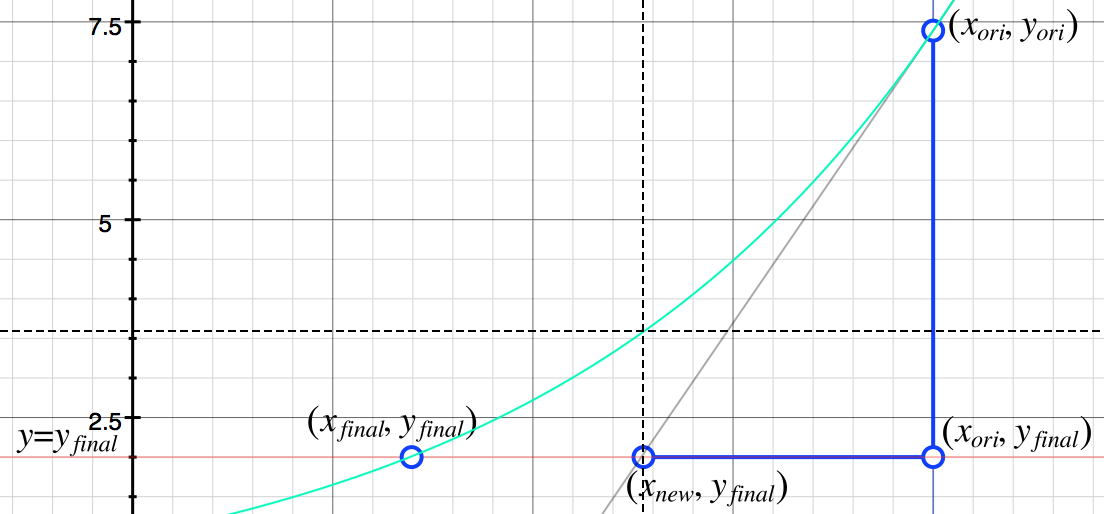
\includegraphics[scale=0.5]{images/牛顿方法示例图片}
		\caption{牛顿方法示例图}
	\end{figure}

	\item 在逻辑回归中使用牛顿方法的过程
	\begin{enumerate}
		\item 由上图可知,$\tan\alpha = \frac{y_{ori}-y_{final}}{x_{ori}-x_{new}} = \frac{f(x_{ori})-f(x_{final})}{x_{ori}-x_{new}} = f'(x_{ori})$\footnote{$\alpha$是切线$y=f'(x_{ori})x + b$与水平线$y=y_{final}$的夹角,不好标就没画出来了},可以得到
		\begin{equation}
			x_{new} := x_{ori} - \frac{f(x_{ori})-f(x_{final})}{f'(x_{ori})}
		\end{equation}
		
		\item 此时,我们得到了一个新的点$(x_{new}, y_{new})$,相比与原来的点$(x_{ori},y_{ori})$,这个点离最终的$(x_{final}, y_{final})$更近了。

		\item 特殊地,在逻辑回归中,我们要得到的是似然函数$l(\theta)$的极值,极值点的导数为$0$。于是,为了在逻辑回归中使用牛顿方法,我们用$l'(\theta)$代替$f(x)$,且$l'(\theta_{final}) = 0$,于是,上式变成
		\begin{align}
			\theta_{new} &:= \theta_{ori} - \frac{l'(\theta_{ori})-l'(\theta_{final})}{l''(\theta_{ori})} \\
			&:=  \theta_{ori} - \frac{l'(\theta_{ori})}{l''(\theta_{ori})}
		\end{align}
		这就是逻辑回归使用牛顿方法时的迭代方式
	\end{enumerate}

	\item 矩阵表达形式 \\
	将上面的式子改写为矩阵表达的形式,如下
	\begin{equation}
		\theta := \theta - H^{-1}\nabla_{\theta}l(\theta)
	\end{equation}
	其中,$H$称为Hessian\footnote{关于Hessian矩阵的介绍请见附录},是一个$n*n$矩阵
	\begin{equation}
		H_{ij} = \frac{\partial^2l(\theta)}{\partial\theta_i\partial\theta_j}
	\end{equation}

	\item 关于牛顿方法的思考
	\begin{enumerate}
		\item 因为不论我们要得到的是最大值还是最小值,其极值点的导数均为$0$,因此,虽然上述逻辑回归中,我们要得到的时似然函数的极大值,但是,若在其他问题中我们要的得到的时极小值,最终的迭代方式还是一样的。
		\item 但是,通过此方法找到的只是极值点(且每次应该只能找到一个解),很可能只是局部最优,如何保证其为全局最优(最大或最小)呢?。{\color{red}{此项待研究。。}}
	\end{enumerate}

	\item 牛顿方法与梯度下降方法的异同
	\begin{enumerate}
		\item 牛顿方法可以在很少的迭代次数就收敛,而梯度下降要收敛需要迭代的次数可能较多
		\item 但是,牛顿方法每次迭代的计算量较大(因为要计算$H^{-1}$),这在特征维度$n$较大时将会耗费较多的性能
		\item 综上,在特征维度$n$不是太大时,使用牛顿方法能够很快就收敛;但是若特征维度$n$很大时,虽然使用牛顿方法需要迭代的次数较少,但是它每次耗费的计算量太大,整个学习的时间不一定能够比梯度下降少。
	\end{enumerate}
\end{enumerate}















		
	\section{广义线性模型}
\subsection{指数分布族}
\begin{enumerate}
	\item 指数分布族的一般形式
	\begin{equation}
		p(y;\eta) = b(y)e^{\eta^T T(y) - a(\eta)}
	\end{equation}
	其中,$\eta$称为natural parameter(自然参数???); \\
	$T(y)$称为sufficient statistic(充分统计量??),大部分情况下,$T(y) = y$,在$T(y)=y$时,$\eta$往往为标量; \\
	$a(\eta)$称为 log partition function;
	\item 
\end{enumerate}

\subsection{线性回归与逻辑回归中,GLMs各部分的值}
主要是讲线性回归于逻辑回归中的式子尽可能地转化成指数分布族的一般形式,然后在根据该一般形式写出$\eta$,$T(y)$,$a(\eta)$的形式。\\
详细过程:略

\subsection{如何构造一般线性模型}




























		\subsection{Softmax Regression}
\subsubsection{关于$\phi$的说明}
\begin{enumerate}
	\item 对于总共有$k$类的分类问题,因为每个分类出现的概率和为1,故仅有$k-1$维特征是相互独立的
	\item 我们将$p(y=i;\phi)$记为$\phi_i$;于是$\phi_k=p(y=k;\phi)=1-\sum_{i=1}^{k-1}\phi_i$。
\end{enumerate}

\subsubsection{关于$T(y)$的表示法说明}
\begin{enumerate}
	\item 为了描述$T(y)$属于多分类问题中的那一类,我们用$k-1$维向量来描述$T(y)$,其中,若$T(y)$属于第$i$类,则第$i$维值为1,其余均为0\footnote{此种表示方法称为One-Hot}。示例如下:
	\begin{equation}
		T(2) = \left[\begin{matrix} 0 \\ 1 \\ 0 \\ \vdots \\ 0 \end{matrix}\right], \quad
		T(1) = \left[\begin{matrix} 1 \\ 0 \\ 0 \\ \vdots \\ 0 \end{matrix}\right], \quad 
		T(k-1) = \left[\begin{matrix} 0 \\ 0 \\ 0 \\ \vdots \\ 1 \end{matrix}\right]
	\end{equation}
	于是,$T(k)$就是个$\vec{0}$向量\footnote{因为它$0\to n-1$维均不是}
	\begin{equation}
		T(k) = \left[\begin{matrix} 0 \\ 0 \\ 0 \\ \vdots \\ 0 \end{matrix}\right]
	\end{equation}
	\item 为了描述方便,我们使用以下新的表示方法
	\begin{enumerate}
		\item $1\{\cdot\}$,在$\cdot$的值为$True$时,$1\{True\}=1$,否则$1\{False\}=0$。如$1\{2=3\}=0$,$1\{2=2\}=1$
		\item 在以上表示法下,$T(y)$可表示成以下形式
		\begin{align}
			\left(T(y)\right)_i &= 1\{y=i\} \\
			& \downarrow \\
			E\left[\left(T(y)\right)_i\right] &= P(y=i)=\phi_i
		\end{align}
	\end{enumerate}
\end{enumerate}

\subsubsection{证明多项式分布属于指数族分布}
\begin{enumerate}
	\item 在多分类问题中,$p(y;\phi)$表示的含义及其表示方式
	\begin{enumerate}
		\item 与逻辑回归时的二分类一样,$p(y=k;\phi)$表示的是取到第$k$类的概率,用$p(y;\phi)$将$p(y=1;\phi), p(y=2;\phi), \dots, p(y=k;\phi)$表示成一个表达式
		\item 参考逻辑回归的方式,我们将$p(y;\phi)$表示为
		\begin{align}
			p(y;\phi) &= \phi_{1}^{1\{y=1\}}\phi_{2}^{1\{y=2\}}\dots\phi_{k}^{1\{y=k\}} \\
			&= \phi_{1}^{1\{y=1\}}\phi_{2}^{1\{y=2\}}\dots\phi_{k}^{1-\sum_{i=1}^{k-1}1\{y=i\}} \\
			&= \phi_{1}^{\left(T(y)\right)_1}\phi_{2}^{\left(T(y)\right)_2}\dots\phi_{k}^{1-\sum_{i=1}^{k-1}\left(T(y)\right)_i} \\
			&= e^{\left(T(y)\right)_1\ln\phi_1 + \left(T(y)\right)_2\ln\phi_2 + \dots + \left(T(y)\right)_{k-1}\ln\phi_{k-1} + \left[1-\sum_{i=1}^{k-1}\left(T(y)\right)_i\right]\ln\phi_k } \\
			&= e^{\left(T(y)\right)_1\ln\frac{\phi_1}{\phi_k} + \left(T(y)\right)_2\ln\frac{\phi_2}{\phi_k} + \dots + \left(T(y)\right)_{k-1}\ln\frac{\phi_{k-1}}{\phi_k} + \ln\phi_k} \\
			&= b(y)e^{\eta^T T(y) - a(\eta)}
		\end{align}
		\end{enumerate}
	\item 从上式可得
	\begin{align}
		b(y) &= 1 \\
		\eta^TT(y) &= \left(T(y)\right)_1\ln\frac{\phi_1}{\phi_k} + \left(T(y)\right)_2\ln\frac{\phi_2}{\phi_k} + \dots + \left(T(y)\right)_{k-1}\ln\frac{\phi_{k-1}}{\phi_k} \\
		&\downarrow \\
		\eta^T &= \left[\begin{matrix}
		\ln\frac{\phi_1}{\phi_k} \\ \ln\frac{\phi_2}{\phi_k} \\ \vdots \\ \ln\frac{\phi_{k-1}}{\phi_k}
		\end{matrix}\right] \\
		a(\eta) &= -\ln\phi_k
	\end{align}
\end{enumerate}


\subsubsection{使用Softmax进行分类}
\begin{enumerate}
	\item 对于$\eta$中的某一项
	\begin{align}
		\eta_i &= \ln{\frac{\phi_i}{\phi_k}} \\
		&\downarrow \\
		e^{\eta_i} &= \phi_i \\
		&\downarrow \\
		\phi_k e^{\eta_i} &= \phi_i \\
		\phi_k\sum_{i=1}^{k}e^{\eta_i} &= \sum_{i=1}^{k}\phi_i = 1 \\
		&\Downarrow \\
		\phi_i &= \phi_k\cdot e^{\eta_i} \\
		&= e^{\eta_i} \cdot \frac{1}{\sum_{j=1}^{k}e^{\eta_j}}
	\end{align}
	如上所示,$\phi_i = \frac{e^{\eta_i}}{\sum_{j=1}^{k}e^{\eta_j}}$称为Softmax函数
	\item 最后,再使用前面的假设三:$\eta_i = \theta_i^Tx, \quad i=1,2, \dots, k-1, \quad \theta_i \in {\rm I\!R}^{n+1}$,可得到
	\begin{align}
		p(y=i|x; \theta) &= \phi_i \\
		&= \frac{e^{\eta_i}}{\sum_{j=1}^{k}e^{\eta_j}} \\ 
		&= \frac{e^{\theta_i^Tx}}{\sum_{j=1}^{k}e^{\theta_j^Tx}}
	\end{align}
	\item 故
	\begin{align}
		h_\theta(x) &= E\left[T(y)|x;\theta\right] \\
		&= E\left[\left[\begin{matrix} 1\{y=1\} \\ 1\{y=2\} \\ \vdots \\ 1\{y=k-1\} \end{matrix}\right|x;\theta\right] \\
		&= \left[\begin{matrix}\phi_1 \\ \phi_2 \\ \vdots \\ \phi_{k-1} \end{matrix}\right] \\ 
		&= \left[\begin{matrix}
		\frac{e^{\theta_1^Tx}}{\sum_{j=1}^{k}e^{\theta_j^Tx}} \\
		\frac{e^{\theta_2^Tx}}{\sum_{j=1}^{k}e^{\theta_j^Tx}} \\
		\vdots \\
		\frac{e^{\theta_{k-1}^Tx}}{\sum_{j=1}^{k}e^{\theta_j^Tx}}
		\end{matrix}\right]
	\end{align}
	如上,最终$h_\theta(x)$可得到$k-1$维向量,通过总概率为1得到第$k$维的概率值,由此可以得到每一种类别的概率值
	\item 以上得到多分类中每种分类概率值的方法就叫做Softmax回归(Softmax Regression)
\end{enumerate}


\subsubsection{参数$\theta$的拟合方式}
使用对数似然估计方法
\begin{align}
	l(\theta) &= \sum_{i=1}^{m}\ln p\left[y^{(i)}|x^{(i)};\theta\right] \\
	&= \sum_{i=1}^{m} \ln \prod_{l=1}^{k}\left[
	\frac{e^{\theta_l^Tx^{(i)}}}{\sum_{j=1}^{k}e^{\theta_l^Tx^{(i)}}}
	\right]^{1\{y^{(i)}=l\}}
\end{align}
{\color{red}{后续待补充}}













	\section{生成学习算法}
\subsection{生成学习算法简介}

\subsubsection{判别学习算法\&生成学习算法}
\begin{enumerate}
	\item 判别学习算法:计算$p(y|x)$,例如逻辑回归中计算$p(y=1|x)$与$p(y=0|x)$
	\item 生成学习算法:计算$p(x|y)$与$p(y)$,然后通过贝叶斯公式$p(y|x) = \frac{p(x|y)p(y)}{p(x)}$计算得到$p(y|x)$
	\begin{enumerate}
		\item 式子中的$p(y)$就是每个$y=k$所占的比例,既然我们有了数据,就可以用其频率当作其比例
		\item 不论$p(y|x)$中$y$的值为多少,式中的$p(x)$均是一样的值(可通过全概率公式计算得到),因此,对于$p(y|x)$较大的$y=k$,$p(x|y)p(y)$也较大,因此,在最优化过程中,可以不计算$p(x)$,于是优化过程变为
		\begin{align}
			arg\max{p(y|x)} &= arg \max_y{\frac{p(x|y)p(y)}{p(x)}} \\
			&= arg\max_y{p(x|y)p(y)}
		\end{align}
		省去了计算$p(x)$的过程
	\end{enumerate}
	
	\item 判别学习算法是给如一系列特征,得到这些特征应该是哪一种结果;生成学习算法学习的是这一种结果应该有什么特征

\end{enumerate}




















		\subsection{高斯判别分析}
以下内容中均假设$p(x|y)$服从多重正态分布(高斯分布)

\subsubsection{多重正态分布简介}
\begin{enumerate}
	\item $n$重正态分布可由均值向量$\mu \in {\rm I\!R}^n$和协方差矩阵$\Sigma \in {\rm I\!R}^{n\times n}$确定,记做$N(\mu, \Sigma)$,表示为:
	\begin{equation}
		p(x; \mu, \Sigma) = \frac{1}{(2\pi)^{\frac{n}{2}}|\Sigma|^\frac{1}{2}}e^{-\frac{1}{2}(x-\mu)^T\Sigma^{-1}(x-\mu)}
	\end{equation}
	其中,$|\Sigma|$是协方差矩阵$\Sigma$的行列式;$\Sigma=\mathrm{Cov}(X) = E(XX^T) - E(X)\left[E(X)\right]^T$,$X$的期望为$E(X) = \int_{x}xp(x;\mu,\Sigma)dx = \mu$
\end{enumerate}

\subsubsection{高斯判别分析模型}
\begin{enumerate}
	\item 高斯判别分析模型针对的是连续性随机变量,如果是离散型随机变量请使用后续会讲到的朴素贝叶斯
	\item 当我们使用高斯判别分析模型是,即有了以下的模型
	\begin{align}
		y & \sim B(1, \phi) = Bernoulli(\phi) \\
		x|y=0 &\sim N(\mu_0, \Sigma) \\
		x|y=1 &\sim N(\mu_1, \Sigma)
	\end{align}
	于是,其概率密度为:
	\begin{align}
		p(y) &= \phi^y(1-\phi)^{1-y} \\
		p(x|y=0) &= \frac{1}{(2\pi)^{\frac{n}{2}}|\Sigma|^\frac{1}{2}}e^{-\frac{1}{2}(x-\mu_0)^T\Sigma^{-1}(x-\mu_0)} \\
		p(x|y=1) &= \frac{1}{(2\pi)^{\frac{n}{2}}|\Sigma|^\frac{1}{2}}e^{-\frac{1}{2}(x-\mu_1)^T\Sigma^{-1}(x-\mu_1)}
	\end{align}
	在上式中,$\phi, \mu_0, \mu_1, \Sigma$就是我们要求的参数(注意,有2个$\mu$,共享1个$\Sigma$),其对数似然函数为:
	\begin{align}
		l(\phi, \mu_0, \mu_1, \Sigma) &= \log \prod_{i=1}^{m} p\left(x^{(i)}, y^{(i)}; \phi, \mu_0, \mu_1, \Sigma\right) \\
		&= \log \prod_{i=1}^{m} p\left(x^{(i)}|y^{(i)}; \mu_0, \mu_1, \Sigma\right)p\left(y^{(i)};\phi\right)
	\end{align}
	注意$p(x|y)$中并没有参数$\phi$,$p(y)$中只有参数$\phi$
	\item 求解似然函数后可得参数如下
	\begin{align}
		\phi &= \frac{1}{m} \sum_{i=1}^{m}1\{y^{(i)=1}\} \\
		\mu_0 &= \frac{\sum_{i=1}^{m}1\{y^{(i)}=0\}x^{(i)}}{\sum_{i=1}^{m}1\{y^{(i)}=0\}} \\
		\mu_1 &= \frac{\sum_{i=1}^{m}1\{y^{(i)}=1\}x^{(i)}}{\sum_{i=1}^{m}1\{y^{(i)}=1\}} \\
		\Sigma &= \frac{1}{m}\sum_{i=1}^{m}\left(x^{(i)}-\mu_{y^{(i)}}\right)\left(x^{(i)}-\mu_{y^{(i)}}\right)^T
	\end{align}
	下面解释下以上各参数表达式的意义: \\
	$\phi$:表示所有数据中$y=1$所占的比例; \\
	$\mu_0$: 其分母表示所有数据中$y=0$的数目,分子表示$y=0$对应的$x$的和;$\mu_1$同理 \\
	$\Sigma$: 协方差矩阵,前面已说过,不再赘述
	\item 说明
	\begin{enumerate}
		\item 使用通过高速判别分析得到的模型得到的是两个高斯分布
		\item 这两个高速分布有共同的协方差$\Sigma$,但是其期望$\mu$不一样,若画出其等高线,在图形上表现为两个等高线形状(由$\Sigma$决定)一样,但是其中心(由$\mu$决定)不一样。
	\end{enumerate}
\end{enumerate}

\subsubsection{高斯判别分析\&逻辑回归}
\begin{enumerate}
	\item 如果我们将$\phi, \mu_0, \mu_1, \Sigma$看出$x$的函数,进行整理后最终可得到
	\begin{equation}
		p(y=1|x; \phi, \mu_0, \mu_1, \Sigma) = \frac{1}{1+e^{-\theta^Tx}}
	\end{equation}
	其中,$\theta$是$\phi, \mu_0, \mu_1, \Sigma$的函数
	\item 如果$p(x|y)$服从多重高斯分布,则$p(y|x)$服从逻辑回归;但反之却不成立,从$p(y|x)$服从逻辑回归无法得到$p(x|y)$服从多重高斯分布。这说明GDA需要更多的条件,其做了更强的假设。
	\item 如果$p(x|y)$确实服从或近似服从高斯分布,那么GDA能够很好地进行预测;在数据集$m$很大时,严格意义上讲在准确率上没有比GDA更好地算法。当然,GDA会比逻辑回归好;甚至在数据集较小时,GDA也往往比逻辑回归好
	\item 因为逻辑回归的假设更弱(可理解为需要的条件更少),因此其具有更好的鲁棒性(可理解为适应能力更好),即使$p(y|x)$并不符合也不近似符合高斯分布,逻辑回归也能较好地预测
\end{enumerate}
















		\subsection{朴素贝叶斯}
\begin{enumerate}
	\item 在GDA中,随机变量$X$是连续的,当随机变量是离散值时,我们使用朴素贝叶斯来进行预测
	\item 朴素贝叶斯举例介绍:以通过邮箱中的文本预测是否为垃圾邮件为例,$y=1$表示该邮件是垃圾邮件
	\begin{enumerate}
		\item 对每封邮件建立词向量\footnote{此处的词向量比较简单,与文本分析(NLP)中的词向量不一样,也不是One-Hot的形式},每个词在向量中占据一个位置,若该词存在,则将该位的值设为1,若不存在则设为0,得到如下向量
		\begin{align}
			x = \left[\begin{matrix}1 \\ 0 \\ 0 \\ \vdots \\ 1 \\ \vdots \\ 0 \end{matrix}\right] \quad
			\begin{matrix}a \\ ad \\ address \\ \vdots \\ buy \\ \vdots \\ zygmurgy \end{matrix}
		\end{align}
		如上所示,该邮件中有a, buy等,没有ad, address, zygmurgy等。
		\footnote{一般来说,建议通过扫描训练集来获取可能出现的词(而不是从字典中获取),这样做一方面可以减小建模时的特征数,节省计算量和存储空间;另一方面还可以避免出现一些字典中没有的词(如CS299,或一些人名等)\\
		另外,还可以将一些无实意、出现频率又比较高的词去除,如a, an, the等}
		\item 若要使用多项式分布来进行预测,按照之前的逻辑回归方式,在词向量维度较多时并不可取(PS:讲义中的$2^{50000}-1$看起来似乎有问题,对$50000$个词建模只需要有$50000+1$个参数,哪来的$2^{50000}-1$??{\color{red}{待研究...}})
		\item 为了更方便地进行建模,我们做了一个假设:假设对于给定的$y$,$x_i$($x_i$指词向量中的第$i$个词)是相互条件独立的,即$p(x_2|y, x_1) = p(x_2|y)$,给定的$x_1$条件并不影响$p(x_2|y)$。此假设称为{\color{blue}{朴素贝叶斯假设}}。由此得到的分类器称为{\color{blue}{朴素贝叶斯分类器}}。
		\item 根据以上假设,我们可以得到以下式子:
		\begin{align}
			p(x_1, \dots, x_n|y) &= p(x_1|y)p(x_2|y, x_1)p(x_3|y, x_1, x_2)\dots p(x_n|y, x_1, x_2, \dots, x_{n-1}) \\
			&= p(x_1|y)p(x_2|y)p(x_3|y)\dots p(x_n|y) \\
			&= \prod_{i=1}^{n}p(x_i|y)
		\end{align}
		\item 与GDA类似,上式由参数$\phi_{i|y=1}=p(x_i=1|y=1)$,$\phi_{i|y=0}=p(x_i=1|y=0)$,$\phi_y=p(y=1)$决定。似然函数可表示为:
		\begin{align}
			L(\phi_y, \phi_{i|y=0}, \phi_{i|y=1}) = \prod_{i=1}^{n}p(x^{(i)}|y^{(i)})
		\end{align}
		\item 通过最大似然估计,可得
		\begin{align}
			\phi_{j|y=1} &= \frac{\sum_{i=1}^{m}1\{x_j^{(i)}=1 \cap y^{(i)}=1\}}{\sum_{i=1}^{m}1\{y^{(i)}=1\}} \\
			\phi_{j|y=0} &= \frac{\sum_{i=1}^{m}1\{x_j^{(i)}=1 \cap y^{(i)}=0\}}{\sum_{i=1}^{m}1\{y^{(i)}=0\}} \\
			\phi_y &= \frac{\sum_{i=1}^{m}1\{y^{(i)}=1\}}{m}
		\end{align}
		其中: \\
		$\cap$表并集,即两个条件同时满足 \\
		$\phi_{j|y=1}$表示出现词$x_j$的垃圾邮件在所有垃圾邮件中所占的比例 \\
		$\phi_{j|y=0}$表示出现词$x_j$的非垃圾邮件在所有非垃圾邮件中所占的比例 \\
		$\phi_y$表示垃圾邮件占所有邮件的比例
		\item 使用贝叶斯公式计算$p(y|x)$
		\begin{align}
			p(y=1|x) &= \frac{p(x|y=1)p(y=1)}{p(x)} \\
			&= \frac{\prod_{i=1}^{n}p(x_i|y=1)p(y=1)}{\left[\prod_{i=1}^{n}p(x_i|y=1)\right]p(y=1)+\left[\prod_{i=1}^{n}p(x_i|y=0)\right]p(y=0)}
		\end{align}
		对$p(y=0|x)$同理,通过比较那个概率更高\footnote{所以,其实$p(x)$并没有必要求,虽然也不难求}来判断是否为垃圾邮件。
		\item 虽然以上过程中只是二分类,但实际上,对于多分类也是以上的套路;
		\item 对于连续型随机变量,也可以对其分段离散化,然后使用朴素贝叶斯进行预测
	\end{enumerate}
\end{enumerate}

\subsection{拉普拉斯平滑}
\subsubsection{背景介绍}
\begin{enumerate}
	\item 在朴素贝叶斯中,若在预测时出现了一个我们训练集中没有的词,那么预测结果为
	\begin{align}
		\phi_{{x_j}|y=1} &= \frac{\sum_{i=1}^{m}1\{x_j^{(i)}=1 \cap y^{(i)}=1\}}{\sum_{i=1}^{m}1\{y^{(i)}=1\}} \\
		&= 0 \\
		\phi_{{x_j}|y=1} &= \frac{\sum_{i=1}^{m}1\{x_j^{(i)}=1 \cap y^{(i)}=0\}}{\sum_{i=1}^{m}1\{y^{(i)}=0\}} \\
		&= 0 \\
		p(y=1|x) &= \frac{\prod_{i=1}^{n}p(x_i|y=1)p(y=1)}{\left[\prod_{i=1}^{n}p(x_i|y=1)\right]p(y=1)+\left[\prod_{i=1}^{n}p(x_i|y=0)\right]p(y=0)} \\
		&= \frac{0}{0}
	\end{align}
	此时出现了$\frac{0}{0}$的情况,没法进行预测。为了解决此问题,我们可以使用拉普拉斯平滑。\footnote{吴恩达的视频中,举了一个已知前面5次比赛都失败,预测第6次失败的概率,可以看下。}
\end{enumerate}

\subsubsection{拉普拉斯平滑介绍}
\begin{enumerate}
	\item $\frac{0}{0}$出现的原因 \\
	由前面$\phi_j = \frac{\sum_{i=1}^{m}1\{z^{(i)}=j\}}{m}$可知,$\phi_j$为出现$z^{(i)}=j$的数据占总数据的比例,在$z^{(i)}=j$在训练集中未出现过时,就会出现$\phi_j=0$\footnote{在$=0$处频数为0,在$=1$处频数也为0},从而导致出现$\frac{0}{0}$的情况,为了解决此问题,我们队$\phi_j$稍作更改:
	\begin{equation}
		\phi_j = \frac{\sum_{i=1}^{m}1\{z^{(i)}=j\}+1}{m+k}
	\end{equation}
	经过此方式处理后:
	\begin{enumerate}
		\item $\sum_{j=1}^{k}\phi_j = 1$仍旧成立
		\item 对任意$\phi_j \neq 0$
	\end{enumerate}
\end{enumerate}















	\section{附录}
\subsection{定义}
\subsubsection{各类变量}
\begin{enumerate}
	\item $i$: 第$i$个数据集,从1开始,截止于m
	\item $j$: 第$j$维特征,从0开始,截止于n
	\item $m$: 数据集大小,共$m$组数据
	\item $n$: 维度大小,共$n$维特征
	\item $i, j, m, n$的关系: $\sum_{i=1}^{m}\sum_{j=0}^{j=n}{\theta_{j}x_j^{(i)}}$
	\item $(x^{(i)}, y^{(j)})$: 第i个训练集
	\item $P(y|x;\theta)$中,$y$做为一个个体;$x:\theta$作为一个个体,表示$x$以$\theta$为参数
\end{enumerate}

\subsubsection{充分统计量}
\begin{enumerate}
	\item 不损失信息的统计量就是充分统计量,它概况了样本中所包含的未知参数的全部信息。
	\item 定义: 设$x_1, x_2, \dots, x_n$是来自某个总体$X$的样本,总体的分布函数为$F(x;\theta)$,若统计量$T=T(x_1, x_2, \dots, x_n)$为$\theta$的充分统计量,则在给定了$T$的取值后,$x_1, x_2, \dots, x_n$的条件分布$P(X_1=x_1, X_2=x_2, \dots, X_n=x_n$与$\theta$无关
	\item 充分统计量不唯一。实际上,样本本身就是参数的一个充分统计量
	\item 因子分解定理{\color{red}{(没看懂)}}: 设总体的概率函数为$p(x;\theta)$,$x_1, x_2, \dots, x_n$是来自总体的样本,则统计量$T=T(x_1, x_2, \dots, x_n)$为充分统计量的充要条件为:
	\begin{equation}
		p(x_1, x_2, \dots, x_n;\theta) = g\left[T(x_1, x_2, \dots, x_n),\theta\right]\cdot h(x_1, x_2, \dots, x_n)
	\end{equation}
	其中,$g(t,\theta)$是通过统计量T的取值而依赖于样本的,而$h(x_1, x_2, \dots, x_n)$不依赖于$\theta$
	\item 更详细内容: http://wenku.baidu.com/view/8813423343323968011c92ed.html
\end{enumerate}

\subsubsection{自然参数}
\begin{enumerate}
	\item 
	\item 
\end{enumerate}


		\section{中英对照表}
\begin{enumerate}
	\item 最小均方 - LMS: Least Mean Squares
	\item 线性回归 - LR: Linear Regression
	\item 逻辑回归 - LR: Logistic Regression
	\item 梯度下降 - GD: Gradient Descent
	\item 随机梯度下降 - SGD: Stochastic Gradient Descent
	\item 局部加权回归 - LWR:Local Weight Regression
	\item 独立同分布 - IID: Independently and Identically Distributed
\end{enumerate}
\end{document}










